\begin{tikzpicture}
    \begin{scope}[shift={(-4,0)}]

        \begin{scope}
            \clip (-1,-2) rectangle  +(2,4);

            \node[inner sep=0pt] at (5.6,-0.)
                {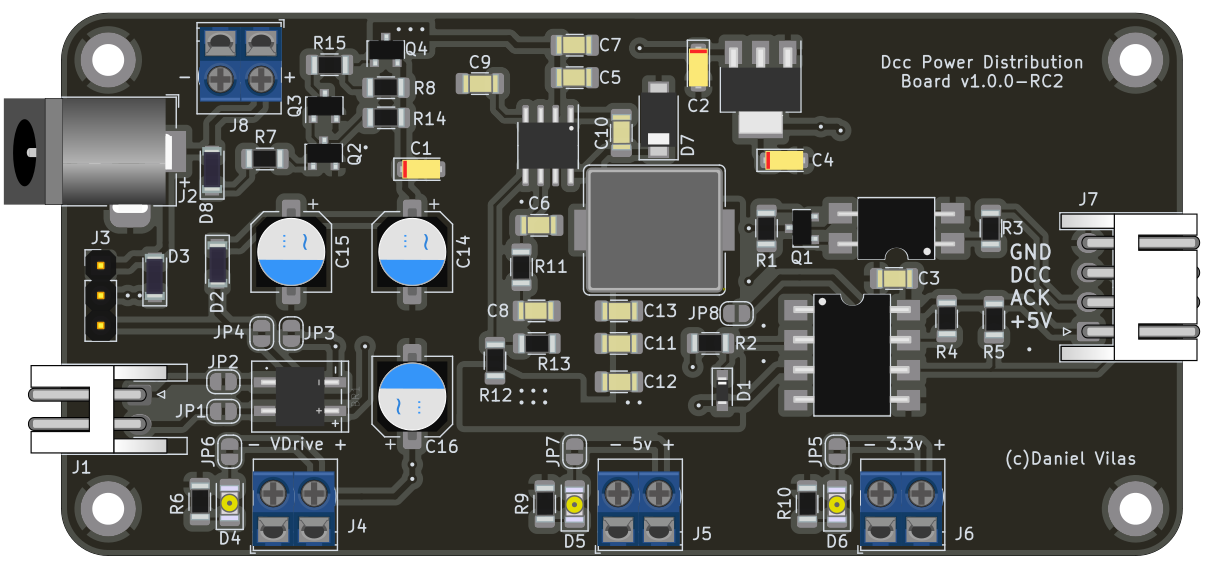
\includegraphics[scale=1.3]{images/front.png}};
        \end{scope}
        \draw[yellow,line width=2pt,rounded corners=4pt] 
            (-0.3,-0.7) rectangle +(0.6,1.4);
        \node[below] at (0,-2) {(a) Automatico};
    \end{scope}

    \begin{scope}
        % \draw [step=0.1,very thin, yellow] (-2,-2) grid (2,2);
        % \draw [step=0.5,very thin, red] (-2,-2) grid (2,2);
        % \draw [very thin, green] (-2,-2) grid (2,2);

        \begin{scope}
            \clip (-1,-2) rectangle  +(2,4);

            \node[inner sep=0pt] at (5.6,-0.)
                {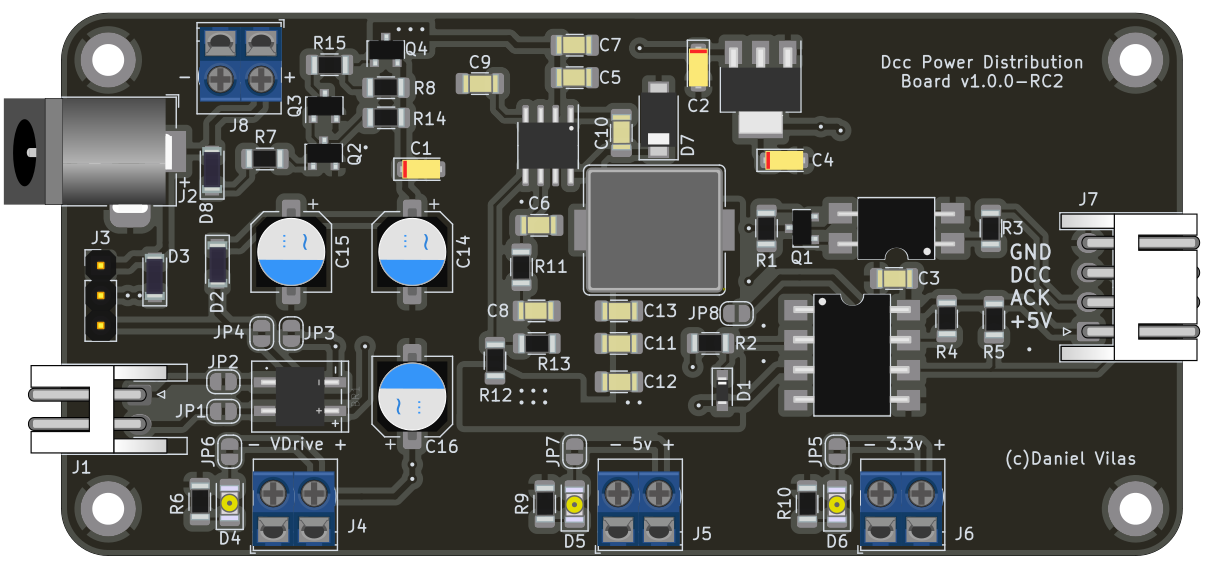
\includegraphics[scale=1.3]{images/front.png}};
        \end{scope}
        %\draw [step=0.1,very thin, yellow] (-0.5,-1) grid +(1,2);
        \draw[yellow,line width=2pt,rounded corners=4pt] 
            (-0.3,-0.7) rectangle +(0.6,1.4);
        \draw[blue, fill=blue!75,line width=1pt]
            (-0.2,0.4) rectangle +(0.35,-.65); 
        \node[below] at (0,-2) {(b) Corriente Continua};
    \end{scope}

    \begin{scope}[shift={(4,0)}]

        \begin{scope}
            \clip (-1,-2) rectangle  +(2,4);

            \node[inner sep=0pt] at (5.6,-0.)
                {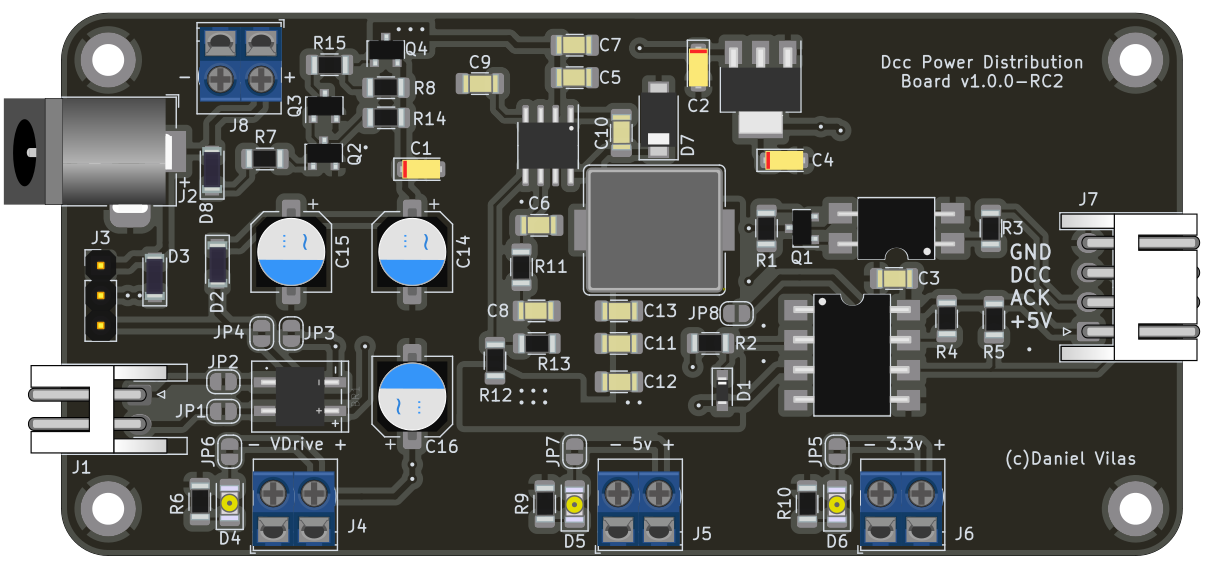
\includegraphics[scale=1.3]{images/front.png}};
        \end{scope}
        %\draw [step=0.1,very thin, yellow] (-0.5,-1) grid +(1,2);
        
        \draw[yellow,line width=2pt,rounded corners=4pt] 
            (-0.3,-0.7) rectangle +(0.6,1.4);

        \draw[blue, fill=blue!75,line width=1pt]
        (-0.2,0.05) rectangle +(0.35,-.65); 
        \node[below] at (0,-2) {(c) DCC};
    \end{scope}
\end{tikzpicture}